\documentclass[11pt, a4paper, ngerman]{article}
\usepackage[utf8]{inputenc}
\usepackage[T1]{fontenc}
\usepackage{lmodern}
\usepackage{amsmath}
\usepackage{amsfonts}
%\usepackage{cm-super} %für scalable Computer Modern font remove!!
\usepackage{amssymb}
\usepackage[]{graphicx} %für bilder und grafiken [draft] damit figuren nicht jedes mal ganz geladen werden
\usepackage[ngerman]{babel} %für die deutsche sprache
\usepackage{authblk} %für \affil
\usepackage{csquotes} %für \enquote
\usepackage{ragged2e} %für bessere flushleft, flushright, center
\usepackage{booktabs} %für Tabellen
\usepackage{fancyhdr} %für Kopf-/Fußzeilen
\usepackage{textcomp} %für mehr Symbole/Zeichen
\usepackage{geometry} %für änderbare Seitenränder
\geometry{
	left=2.5cm,
	right=2.5cm,
	top=2.5cm,
	bottom=2cm,
}
\usepackage{caption} %für leere captions
\usepackage{multicol} %für mehrere Spalten
\usepackage{float} %für Floats out of par, z.B. in minipages
\usepackage{tabularx} %für autmatische Tabbelen Spallten Größen & Umbrüche
\usepackage{array} %für erweiterte tabular format optionen
\usepackage{microtype} %für bessere Abstandsverteilung und Verhindern von durch neue Zeilen abgeschnittenen Wörtern
%\usepackage{tikz} %für Malerei


\usepackage{hyperref} %für verlinktes Inhaltsverzeichnis
\hypersetup{
	hidelinks=true,
	linktoc=all,     %set to all if you want both sections and subsections linked
}

\captionsetup{
	font=small
}
\newcommand*{\vcenteredhbox}[1]{\begin{tabular}{@{}c@{}}#1\end{tabular}} %Für Abbildung mit Textkasten

\title{\textbf{\Huge KI in der Musik – Computer lernen komponieren}}
\date{}
\author[]{\textbf{\LARGE Alexander Reimer und Matteo Friedrich}}
\affil[]{\textbf{\huge Gymnasium Eversten Oldenburg} \\ \vspace{10mm} \textbf{\Large Betreuer: Herr Dr. Glade \& Herr Husemeyer}}

\fancyhf{}
\pagestyle{fancy}
\fancyhead[R]{SCHÜLER EXPERIMENTIEREN - PROJEKTBERICHT}
\fancyfoot[C]{\thepage}
\begin{document}
\setcounter{figure}{1}
\maketitle
\newpage
\tableofcontents
\newpage
\section{Kurzfassung}
In unserem Projekt haben wir eine künstliche Intelligenz (KI) programmiert, die Komponieren lernen soll. Dafür haben wir die Programmiersprache Julia verwendet. Wir haben herausgefunden, dass Machine Learning fast immer mit neuronalen Netzwerken funktioniert. Ein neuronales Netz ist eine Ansammlung von, in mehrere Layer unterteilten, Neuronen. Die Neuronen haben eine Aktivierung und sind mit Gewichten verbunden. Die Aktivierung eines Neurons setzt sich aus den Aktivierungen des vorherigen Layers und den damit verbundenen Gewichten zusammen. Der erste Layer ist der Input Layer. Bei diesem werden die Aktivierungen der Neuronen von Daten bestimmt, z.B. den Pixeln eines Bildes.

Damit die KI nun lernen kann, benötigt sie Trainingsdaten. Diese bestehen aus Paaren von Inputs und den richtigen Outputs dafür (z.\,B. ein Text und die dazugehörige Textart). Durch sie weiß das Programm, wie ein Netzwerk verändert werden muss, und kann die Leistung eines neuronalen Netzwerkes überprüfen, indem es die Cost berechnet. Um die Cost zu berechnen, haben wir die MSE-Funktion benutzt. Es gilt: Die Cost ist die Summe der Fehler eines neuronalen Netzwerkes, d.\,h., niedrigere Cost = besseres Netzwerk.

Die KI lernt nun, indem die Gewichte des Netzwerks optimiert werden, das heißt, sie werden so verändert, dass das Netzwerk eine möglichst kleine Cost hat. Um das Netzwerk zu optimieren, nutzen wir Backpropagation.

Anschließend haben wir Midi-Dateien aus dem Internet heruntergeladen und mit Hilfe von ihnen Trainingsdaten erzeugt. In den Trainingsdaten sind 10 aufeinander folgende Töne eines Liedes als Inputs und der, auf den 10. Ton folgende Ton, als richtiger Output angegeben.
Am Ende haben wir ein neuronales Netzwerk mit Hilfe dieser Trainingsdaten optimiert. Dieses Netzwerk haben wir genutzt, um neue Lieder zu komponieren. Das Ergebnis war sehr enttäuschend, weil die Ergebnisse für das menschliche Gehör zufällig und nicht schön wirkten. Bei einfacheren Tests hat das Programm jedoch gut funktioniert.

Wir haben auch mehrere Möglichkeiten gefunden, unser Netzwerk zu verbessern. Wir hatten außerdem noch eine andere Idee, wie auf unserem Projekt aufbauen könnte.
\newpage

\section{Einleitung} \label{Einleitung}
\textbf{Die Forscherfrage:}\\[1ex]
Wir haben es uns als Ziel gesetzt, eine Künstliche Intelligenz zu programmieren, die man mithilfe von Liedern eines Genres trainieren kann, eigene Lieder zu komponieren. Der Grund dafür ist, dass wir uns für Machine Learning interessieren, da es heutzutage eine sehr wichtige Technologie ist, aber trotzdem nur von wenigen verstanden wird. Dafür wollten wir mit Hilfe der Programmiersprache Julia ein eigenes neuronales Netzwerk erstellen und trainieren. Wir haben uns für den Themenbereich Musik entschieden, weil wir es spannend fanden, dass Computer etwas so menschliches wie Musik verstehen und verarbeiten können. Besonders wichtig war es uns dabei, die Teile des Programms über neuronale Netzwerke und Machine Learning selbst zu schreiben, ohne bereits fertige Lösungen zu benutzen. Sachen wie das grafische Darstellen von Daten und das Auslesen von Midi-Dateien innerhalb von Julia haben wir jedoch aus dem Internet kopiert.

\section{Methode und Vorgehensweise} \label{Methode und Vorgehensweise}
	\subsection{Materialien}
	Für unser Projekt haben wir folgende Materialien/Applikationen verwendet:
	\begin{itemize}
		\item Hardware
		\begin{itemize}
			\item Verschiedene Computer
		\end{itemize}
		\item Software
		\begin{itemize}
			\item Julia, eine objektorientierte, schnelle, dynamische und übersichtliche Programmiersprache, die speziell für mathematische Berechnungen und Datenverarbeitung ausgelegt ist
			\item Julia Packages:
			\begin{itemize}
				\item \hyperref[src:midi]{MIDI}, um mit Musikdateien und Noten zu arbeiten
				\item \hyperref[src:pyplot]{PyPlot}, um Plots darzustellen
				\item \hyperref[src:jld]{JLD}, um Netzwerke und Plots zu speichern
			\end{itemize}
		\end{itemize}
		\item Midi-Dateien zum Trainieren und Testen:
		\begin{itemize}
			\item \href{https://bitmidi.com/}{https://bitmidi.com/}
			\item \href{https://www.midiworld.com/files/}{https://www.midiworld.com/files/}
		\end{itemize}
	\end{itemize}
	\subsection{Vorgehensweise} \label{Vorgehensweise}
		\subsubsection{Struktur und Forward Pass -- Theorie} \label{Struktur und Forwardpass - Theorie}
		Zuerst wollten wir die Grundstruktur eines neuronalen Netzwerkes programmieren. Nach einiger Recherche haben wir herausgefunden, dass ein neuronales Netzwerk aus drei Teilen besteht: dem Input Layer, den Hidden Layers und dem Output Layer [\hyperref[src:1]{1}, \hyperref[src:2]{2}, \hyperref[src:2]{3}].
		
		Der Input Layer ist nur eine Liste aus Zahlen zwischen 0 und 1. Er gibt an, welche Eingaben (Inputs) das Netzwerk bekommen soll, z.\,B. ein Schwarz-Weiß-Bild oder ein Text.
		
		Die Hidden Layers sind eine Ansammlung von in mehrere Layer (Schichten) unterteilten Neuronen. Jedes Neuron besitzt eine Aktivierung (Activation), die als Zahl zwischen 0 und 1 angegeben werden kann, und einen Bias (Verzerrung), der eine beliebige Zahl sein kann. Die Neuronen verschiedener Layer sind alle durch sogenannte Gewichte (Weights) verbunden, die ebenfalls einen beliebigen Wert haben können. Um nun die Aktivierungen eines Neurons zu berechnen, gibt es den sogenannten Forward Pass. Dabei beginnt man im ersten Hidden Layer damit, für alle Neuronen den sogenannten Netz Input (auch net input) zu berechnen. Um den Netz Input eines Neurons zu berechnen, werden alle Aktivierungen des vorherigen Layers mit den von dem Neuron dorthin führenden Gewichten multipliziert und summiert. Der Bias ist eigentlich auch ein Gewicht, jedoch ist er mit einem Neuron verbunden, das IMMER die Aktivierung ($a_i$) 1 hat, weshalb man einfach $+b_i$ statt $+b_i*a_i$ rechnen kann.
		Um aus diesem Netz Input nun die Aktivierung zu berechnen, benötigt man eine Aktivierungsfunktion, die dafür sorgt, dass die Aktivierung zwischen 0 und 1 liegt. Wir haben dafür eine Sigmoidfunktion benutzt, die eine Zahl nimmt und einen Wert zwischen 0 und 1 ausgibt [\hyperref[src:2]{2}]:
		\begin{center}
			\vcenteredhbox{\begin{minipage}{0.4\textwidth}
				{\Large
				\[sig(x)=\frac{1}{1+e^{-x}}\]
				\[a_i=sig\left({netzinput}_i \right)\]}
				wobei $a_i$ = die Aktivierung des Neurons $i$ und $netzinput_{i}$ = der Netzinput des Neurons $i$.
			\end{minipage}}
			\hspace{1em}
			\vcenteredhbox{
			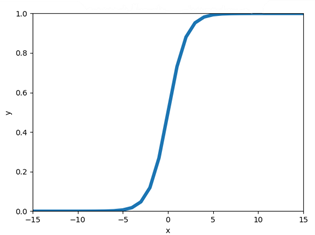
\includegraphics[width=0.5\textwidth]{"pictures/sig_func.png"}\\[0.75ex]
			{\small Abbildung \thefigure: Unsere Sigmoidfunktion}
			}
		\end{center}
		
		Dies wird dann für jedes Neuron in jedem Layer wiederholt. Da man aber immer die Aktivierungen des vorherigen Layers benötigt, muss man das ganze vom Input Layer zum Output Layer machen. Daher auch der Name Forward Pass. Die Outputs sind dann lediglich die Aktivierungen der Neuronen im Output Layer, die Interpretation dieser hängt von den Trainingsdaten ab (s. \hyperref[Backpropagation - Theorie]{Backpropagation -- Theorie)}.
		Die allgemeine Formel für die Aktivierung eines Neurons lautet also:
		
		{\Large \[a_{j} = sig\left(\sum_{L} (a_{L} * W_{Lj}) + b_{j}\right)\]}
		
		\noindent wobei $a_j$ = die Aktivierung des Neurons $j$, $L$ = der nächste Layer, $a_L$ = alle Aktivierungen des Layers $L$ , $W_{Lj}$ = alle Gewichte zwischen dem Neuron $j$ und den Neuronen des Layers $L$, und $b_j$ = der Bias des Neurons $j$.\\[2ex]
		\begin{minipage}{\textwidth}
		\textbf{Eine Beispielrechnung für ein winziges Netzwerk:}%\\[1ex]
			\begin{multicols}{2}
				\begingroup
				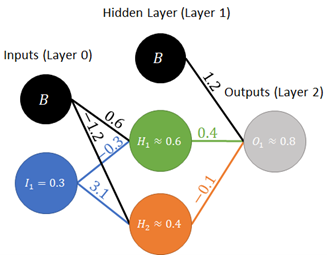
\includegraphics[width=0.5\textwidth]{"pictures/bsp_net_small.png"}
				\captionof{figure}{Ein einfaches Beispiel für ein neuronales Netzwerk mit 3 Layern (Input, Hidden, und Output Layer), 4 Neuronen und 2 \enquote{Bias}-Neuronen. Die Neuronen sind durch Kreise mit der jeweiligen Aktivierung abgebildet. Die Linien zeigen die Verbindungen zwischen den Neuronen mit den dazugehörigen Gewichten. Die schwarzen Kreise zeigen die Bias-Neuronen, deren Aktivierung immer 1 ist.}
				\endgroup
			\columnbreak
				\begin{flushleft}
					$
					\begin{aligned}
						H_1(netzinput) & = 0.3 * (-0.3) + 0.6\\
						& = 0.51
					\end{aligned}
					$\\[2ex]
					$
					\begin{aligned}
						H_1(Aktivierung) & = sig(0.51)\\
						& \approx0.62480647				
					\end{aligned}
					$\\[2ex]
					$H_2(netzinput)=0.3*3.1+(-1.2)=-0.27$\\[2ex]
					$H_2(a)=sig(-0.27)\approx0.432907$\\[2ex]
					$
					\begin{aligned}
						O_1(ni)& \approx0.4*0.62+(-0.1)*0.43+1.2\\
						& =1.406631880283917
					\end{aligned}
					$\\[2ex]
					$O_1(a)=0.803234159160199$
				\end{flushleft}
				\textbf{Ergebnis: [0.803234159160199]}
				\vfill
				\phantom{o}
			\end{multicols}
		\end{minipage}\\[1.25ex]
		
		Jedoch ist das Beispiel ein sehr kleines Netzwerk, das so in der Praxis nicht angewendet werden würde. Neuronale Netzwerke können (theoretisch) unendlich groß sein und die Anzahl der Gewichte vergrößert sich schon bei ein paar zusätzlichen Neuronen drastisch:\\
		
		\begingroup
		\centering
		\noindent 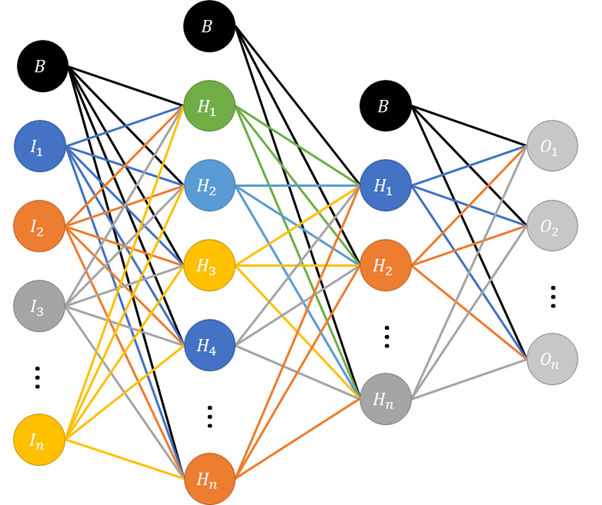
\includegraphics[width=0.5\textwidth]{pictures/bsp_net_big.png}
		\captionof{figure}{Ein größeres neuronales Netzwerk mit 4 Layern}
		\endgroup

		\subsubsection{Struktur und Forward Pass -- Umsetzung} \label{Struktur und Forward Pass - Umsetzung}
		Um die Struktur eines neuronalen Netzwerkes in Julia umzusetzen, haben wir sogenannte \mbox{\textit{Mutable Structs}} benutzt. Mit diesen kann man eigene Datentypen definieren, die selbst erstellte \enquote{Felder} haben. Hier am Beispiel eines Datentyps zum Speichern eines Neurons:\\[1.5ex]
		\begin{minipage}{\textwidth}
			\texttt{mutable struct Neuron\\
			\hspace*{4ex}netinput::Float64\\
			\hspace*{4ex}activation::Float64\\
			\hspace*{4ex}$\delta$::Float64\\
			end}
		\end{minipage}\\[1.5ex]
		Nachdem so ein Datentyp einmal definiert wurde, kann man ganz einfach mit z.B. \mbox{Neuron.activation} auf die Aktivierung oder \mbox{Neuron.netinput} auf den Netz Input zugreifen.
		
		Man kann Mutable Structs auch ineinander verschachteln, was wir ausgenutzt haben, um unsere Netzwerkstruktur zu erstellen.\\[1.5ex]
		\begin{minipage}{\textwidth}
			\textbf{Neuronales Netzwerk vom höchsten bis zum niedrigsten Level:}\\[1ex]
			\underline{network} \textrightarrow Das gesamte neuronale Netzwerk
			\begin{itemize}
				\item allInputs (als Array von Float) \textrightarrow Input Layer
				\item allLayers (als Array von Layer) \textrightarrow Alle Layer des Netzwerkes außer Inputs\\\underline{Layer} \textrightarrow Ein Layer
				\begin{itemize}
					\item neurons (als Array von Neuron) \textrightarrow Alle Neuronen eines Layers\\\underline{Neuron} \textrightarrow Ein Neuron
					\begin{itemize}
						\item netinput (als Float) \textrightarrow Der Netzinput eines Neurons
						\item activation (als Float) \textrightarrow Die Aktivierung eines Neurons
						\item $\delta$ (als Float) \textrightarrow Der $\delta$-Wert des Neurons
					\end{itemize}
				\end{itemize}
				\item allWeights (als Array von einem 2D Array von Float) \textrightarrow alle Weights 
			\end{itemize}
		\end{minipage}\\
	
		Mithilfe der von uns programmierten Funktion \texttt{createNetworkStructure(...)} können wir ganz einfach ein neuronales Netzwerk mit beliebig vielen und großen Layern erstellen. Wie üblich werden die Gewichte und Biases mit zufälligen Werten initialisiert, die in unserem Fall zwischen -2 und 2 liegen. Mit der Funktion \texttt{forwardPass(inputs...)} kann man ganz einfach alle Aktivierungen des Netzwerkes berechnen.
		
		\subsubsection{Backpropagation -- Theorie} \label{Backpropagation - Theorie}
		Doch woher weiß man, welche Werte die Gewichte und Biases haben sollen? Immerhin haben normale Netzwerke tausende von Gewichten und Biases, deren Verbindungen meist für Menschen nicht nachvollziehbar sind.
		
		Nach einiger Recherche im Internet sind wir auf ein Optimierungsverfahren gestoßen: Backpropagation (auch Backward Pass genannt), letztendlich eine effizientere und vergleichsweise einfach anwendbare Version des Gradient Descents, mit der das lokale Minimum gefunden werden kann. Für Backpropagation muss das Programm jedoch wissen, wie gut eine bestimmte “Konfiguration” (Gewichte und Biases) des Netzwerkes ist. Dafür gibt es die sogenannte Cost-Funktion (auch Loss-Funktion genannt), die mithilfe von Trainingsdaten funktioniert. Trainingsdaten bestehen aus einer Liste aus Trainingsdatensätzen. Jeder dieser Datensätze beinhaltet Inputs für das Netzwerk und die richtigen Outputs dafür. [\hyperref[src:1]{1}, \hyperref[src:2]{2}] Machine Learning, das mit solchen Trainingsdaten arbeitet, wird Supervised Learning genannt. [\hyperref[src:1]{1}] In diesen Datensätzen liegt meist auch die Schwierigkeit von Machine Learning (s. \hyperref[Vorgehensweise]{Konfiguration der Trainingsdaten}).
		
		Die Funktion für die Cost des Output Layers und somit gesamten Netzwerkes (für einen Trainingsdatensatz) lautet wie folgt [\hyperref[src:2]{2}]:
		
		{\Large \[C_{0} = \left(a_{L} - y \right)^{2} \]}
		
		\noindent wobei $C_0$ = die Cost des Output Layers, $L$ = der letzte Layer (Output Layer), $a^{(L)}$ =  die Aktivierungen des Layers $L$, und $y$ = die richtigen Outputs für die Inputs, mit denen die Aktivierungen berechnet wurden.
		
		Um die Cost zu berechnen, muss man also für alle Output Neuronen die Differenz der gegebenen und der richtigen Aktivierungen bilden. Danach muss man diese Differenzen quadrieren und am Ende alle Ergebnisse aufsummieren. Dies kann man für alle Trainingsdatensätze wiederholen und von allen Costs den Durchschnitt nehmen, um die allgemeine Performance eines Netzwerkes zu überprüfen. Diese Art der Cost-Funktion wird Mean Squared Error (MSE) genannt. Zusammenfassend kann man also sagen, dass die Cost die Abweichung von den berechneten und den richtigen Outputs angibt.
		
		Aufgrund des Trainingsdatensatzes weiß man nun, wie der Output Layer verändert werden muss.\\
		\begin{minipage}{\linewidth}
			\centering
			\begin{minipage}{0.3\linewidth}
				\begin{figure}[H]
					
\includegraphics[width=1.15\linewidth]{pictures/num_4}
					\caption{Eine handgeschriebene $4^{\hyperref[src:num_4]{[6]}}$}
					\label{fig:num_4}
				\end{figure}
			\end{minipage}
			\hspace{0.05\linewidth}
			\begin{minipage}{0.6\linewidth}
				\captionof{table}{Beispielhafte Outputs eines untrainierten neuronalen Netzwerkes mit Abbildung \ref{fig:num_4} als Input, und die richtigen Outputs dafür – also ein Trainingsdatensatz}
				\begin{tabularx}{\linewidth}{X|l|l|l}
					{entspricht der Zahl} & {Output} & {richtiger Output} & {ändern um:}\\
					\noalign{\hrule height 1.25pt}
					$0$ & $0.867$ & $0.0$ & $-0.867$\\
					\hline
					$1$ & $0.598$ & $0.0$ & $-0.598$\\
					\hline
					$2$ & $0.0012$ & $0.0$ & $-0.0012$\\
					\hline
					$3$ & $1.0$ & $0.0$ & $-1.0$\\
					\hline
					$4$ & $0.386$ & $1.0$ & $+0.614$\\
					\hline
					$5$ & $0.81$ & $0.0$ & $-0.81$\\
					\hline
					$6$ & $0.9976$ & $0.0$ & $-0.9976$\\
					\hline
					$7$	& $0.0$	& $0.0$	& $+0.0$\\
					\hline
					$8$	& $0.754$ & $0.0$ & $-0.754$\\
					\hline
					$9$	& $0.6$ & $0.0$	& $-0.6$\\
				\end{tabularx}
			\end{minipage}
		\end{minipage}\\[2ex]\par
		Doch wie verändert man nun die Aktivierungen des Output Layers? Es müssen alle Gewichte und Biases davor angepasst werden. Um nun zu wissen, wie ein Gewicht verändert werden muss, gibt es folgende Funktion [\hyperref[src:3]{3}]:
		
		{\Large \[\Delta W_{ij} = \epsilon * \delta_i * a_j\]}
		
		\noindent wobei ${\Delta W}_{ij}$ = um wie viel das Gewicht $W$ zwischen den Neuronen $j$ und $i$ verändert werden muss, $\epsilon$ = die Lernrate (meist ein kleiner Wert wie $0.001$), $\delta_i$  $\approx$ die Ableitung der Cost des Neuronen $i$ im Verhältnis zum Weight $W_{ij}$, und $a_j$ = die Aktivierung des Neurons $j$. Was dabei oft verwirrend ist: $j$ bezeichnet das Neuron, welches zuerst kommt, und $i$ das Neuron, welches danach kommt (Reihenfolge im Forward-Pass), obwohl es bei $W_{ij}$ andersherum steht.
		
		Für den Bias wird die gleiche Formel benutzt, mit der Ausnahme, dass $a_j$ immer $1$ ist und so wegfällt. Der Grund dafür liegt darin, dass der Bias, wie in der Struktur beschrieben, eigentlich nur ein Gewicht ist, das mit einem Neuron verbunden ist, welches immer eine Aktivierung von eins hat.
		
		Um nun $\delta_i$ für den Output Layer zu berechnen, gibt es folgende Gleichung [\hyperref[src:3]{3}]:
		
		{\Large \[\delta_{i} = sig'({netzinput}_{i}) * (a_{i}(soll) - a_{i}(ist))\]}
		
		\noindent wobei $sig'(x)$ = die Ableitung von $sig(x)$, also $sig'(x)$ = $sig(x) * (1-sig(x))$, ${netzinput}_i$ = der Netzinput des Neurons $i$ , $a_{i}(soll)$ = die Aktivierung, die das Neuron haben sollte (also das gleiche wie $y$), und $a_{i}(ist)$ = die Aktivierung, die das Neuron hat.
		
		Mit dieser Formel wird berechnet, welche Aktivierung das Neuron haben sollte, was an $(a_{i}(soll)-a_{i}(ist))$ erkennbar ist. Die Aktivierungsfunktion mit dem Netz Input wird als Faktor mit einberechnet, da möglichst nur die Gewichte stark verändert werden sollen, die bei dem Trainingsdatensatz eine hohe Aktivierung haben, also durch diese Inputs besonders angesprochen werden. So werden zum Beispiel beim Sortieren nur die Neuronen miteinander verknüpft, die für ein bestimmtes Muster verantwortlich sind.
		
		Für die Neuronen der Hidden Layers muss man alle $\delta$'s des nächsten Layers mit den von dem Neuron dorthin führenden Weights multiplizieren und dann summieren [\hyperref[src:3]{3}]. Dadurch werden die Änderungen, die die Aktivierungen dieser Neuronen brauchen ($\delta$), zusammengerechnet, da natürlich die Aktivierungen im nächsten Layer unterschiedliche Änderungen in dem gleichen Neuron benötigen. Durch die Multiplikation mit den dahin führenden Weights werden diese Änderungen gewichtet, da sie auf einige Neuronen größere Auswirkungen haben als auf andere. Wie beim Output Layer auch wird diese Summe noch mit $sig'(netzinput)$ multipliziert, um die Aktivierung durch bestimmte Muster angesprochener Neuronen noch weiter zu erhöhen und weniger/kaum angesprochener Neuronen zu senken, sodass die Ergebnisse besser und eindeutiger werden. Die Formel [\hyperref[src:3]{3}]:
		
		{\Large \[sig'({netzinput}_i) * \sum_{L}{\left(\delta_L\ast W_{Li}\right)}\]}
		
		\noindent wobei $L$ = der nächste Layer, $\delta_L$ = alle $\delta$'s des Layers $L$, und $W_{Li}$ = alle Weights, die ein Neuron des nächsten Layers und Neuron $i$ verbinden.
		
		Da immer die nächsten Layer und der Output Layer benötigt werden, ergibt es Sinn, diese Optimierung beim Output Layer zu starten und dann rückwärts die \mbox{$\delta$-Werte} für jeden Layer zu berechnen und für die nächsten Berechnungen zu speichern -- daher auch der Name Backpropagation.
		
		\subsubsection{Konfiguration der Trainingsdaten}
	Die Trainingsdaten für ein neuronales Netzwerk zu finden ist einer der schwierigsten Teile, denn wenn man diese automatisch generieren könnte, wäre keine KI mehr notwendig. Also müssen diese Trainingsdaten oft von Menschen erstellt werden. Das Problem: Um gut trainiert zu werden, benötigen neuronale Netzwerke tausende Trainingsdatensätze. Für Musik ist das einfacher, weil es schon sehr viele Lieder gibt.

	Nach einiger Recherche wurde klar, dass wir die KI keine eigenen Lieder komponieren lassen können, denn dann könnten wir das Machine Learning nicht mit Supervised Learning, also Trainingsdaten, die die richtigen Outputs für bestimmte Inputs enthalten, durchführen, sondern müssten auf Reinforcement Learning zurückgreifen, das heißt, nach jedem Trainingsdatensatz, für alle Wiederholungen der Backpropagation, müsste sich ein Mensch das erzeugte Lied anhören und es bewerten. Das wäre nicht realistisch machbar. (s. \hyperref[Diskussion]{Diskussion} für Unsupervised Learning als Alternative)
	
	Also sind wir stattdessen auf die Idee gekommen, das neuronale Netzwerk immer nur eine weitere Note bestimmen zu lassen, nachdem es $x$ viele vorherige als Inputs bekommen hat. Denn diese könnte man automatisch kontrollieren, da man ja die nächste Note in einem Lied kennt. Und sobald das Netzwerk gut genug trainiert ist, kann man es auch neue Noten über die des originalen Liedes hinaus bestimmen lassen, sodass auch \enquote{originale}, neue Teile komponiert werden.
	
	Das große Problem hierbei ist die Tatsache, dass neuronale Netzwerke nur Zahlen als Input oder Output bekommen können. Deshalb mussten wir eine Möglichkeit finden, einzelne Noten in Zahlen umzuwandeln. Um eine gute Umwandlungsmethode zu finden, mussten wir zuerst definieren, was eine gute Konfiguration einer Note ausmacht. Damit ein neuronales Netzwerk gut mit einem Trainingsdatensatz lernen kann, sollte dieser nicht zu lang sein, weil sonst zu viele Gewichte angepasst werden müssen. Außerdem sollten kleine Änderungen in der Konfiguration auch nur kleine Auswirkungen auf die zugehörige Note haben, weil ein neuronales Netzwerk meistens eine kleine Fehlerquote hat.
	
	Am Ende hatten wir uns dazu entschieden, die Tonhöhe, die Dauer, die der Ton erklingt, und die Position relativ zum vorherigen Ton in unsere Konfiguration einzubauen. Da Ungenauigkeiten bei zum Beispiel der Dauer von kurzen Noten schlimmer sind als von langen Noten, haben wir diese Werte logarithmisch umgewandelt.
		
		\subsubsection{Darstellung der Funktionsweise des Programms}
		\begin{figure}[h]
			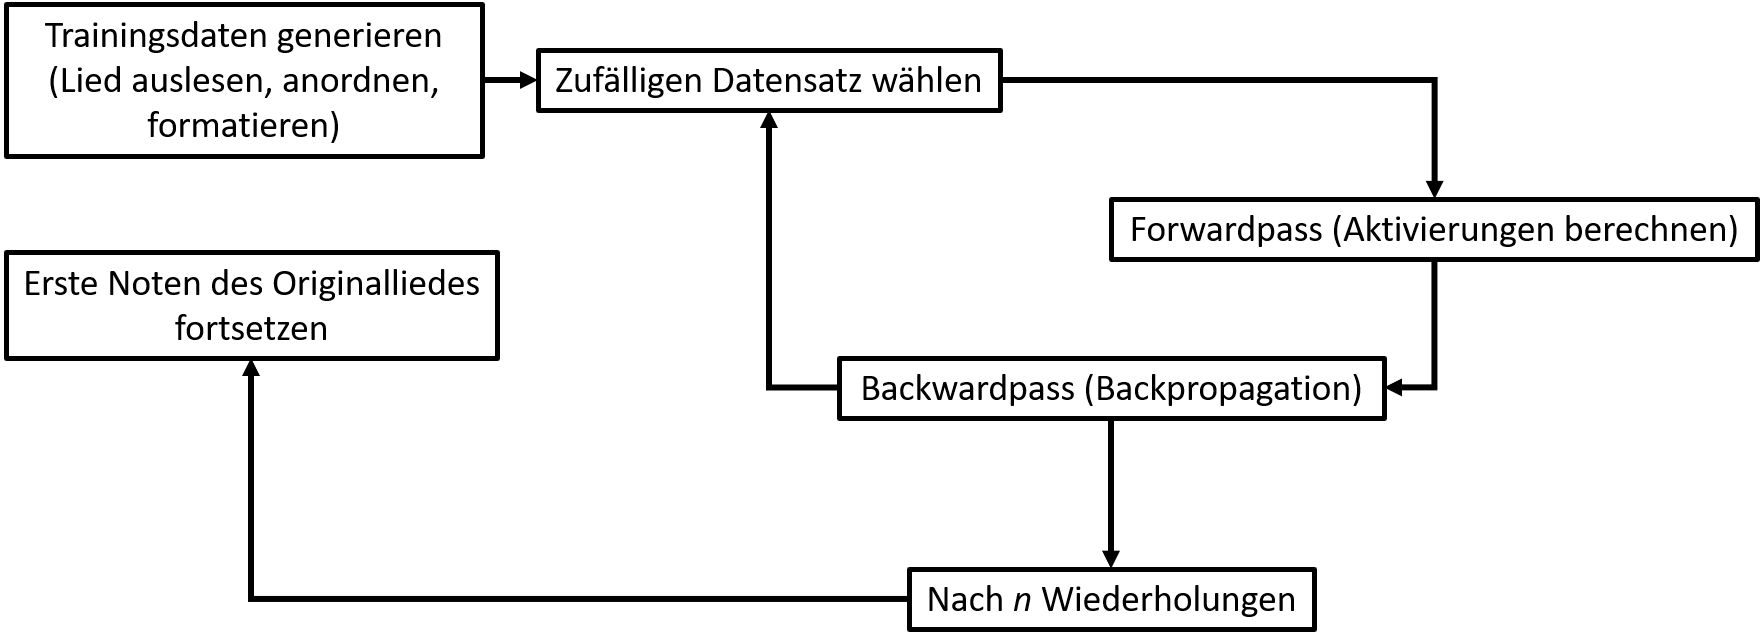
\includegraphics[width=\linewidth]{"pictures/program_schematic.png"}
			\caption{Die grobe Funktionsweise unseres Programms} \label{fig:program}
		\end{figure}
		\subsubsection{Symbole/Syntax -- Verzeichnis}
		Die wichtigsten Symbole:\\[2ex]
		\begin{minipage}{\textwidth}
			\begingroup
			\captionof{table}{Verzeichnis der wichtigsten verwendeten Symbole}
			\begin{tabularx}{\linewidth}{r|X}
				Symbol & Bedeutung\\
				\noalign{\hrule height 1.25pt}
				$a_i$ & Die Aktivierung des Neurons $i$ \\
				\hline
				$b_i$ & Der Bias des Neurons $i$\\
				\hline
				${netzinput}_i$ & Der Netzinput des Neurons $i$\\
				\hline
				$a_L$ & Alle Aktivierungen des Layers $L$\\
				\hline
				$W_{Lj}$ & Alle Gewichte zwischen dem Neuron $j$ und den Neuronen des Layers $L$\\
				\hline
				$W_{ij}$ & Das Gewicht zwischen den Neuronen $i$ und $j$. $j$ bezeichnet das Neuron, welches zuerst kommt, und $i$ das Neuron, welches danach kommt (Reihenfolge im Forward-Pass), obwohl es bei $W_{ij}$ andersherum steht.\\
				\hline
				$C_0$ & Die Cost des Output Layers\\
				\hline
				$\epsilon$ & Die Lernrate (meist ein kleiner Wert wie 0.001)
			\end{tabularx}
			\endgroup
		\end{minipage}\\[2ex]
\section{Ergebnisse}
	Der ganze Code (mit englischen Kommentaren) kann unter \href{https://github.com/AR102/JuFo2021}{https://github.com/AR102/JuFo2021} gefunden werden.
	\subsection{Teilbarkeit -- Erster Testversuch}
	Zuerst haben die Formeln der Backpropagation in Julia als Funktionen eingebaut und eine Variable $\epsilon$ definiert, die für die Lernrate steht. Um das Programm zu testen, haben wir die temporäre Funktion \texttt{generateTrainingData(\ldots)} implementiert, die die nötigen Trainingsdaten ausgibt, um ein neuronales Netzwerk darauf zu trainieren, die Teilbarkeit von Zahlen durch 2 zu überprüfen.
	
	Unser erstes Netzwerk dafür hatte folgende Konfiguration:\\[1.5ex]
	\begin{tabularx}{\linewidth}{lll}	
		Inputs & Hidden & Outputs\\
		32 & 6 & 1
	\end{tabularx}\\[1.5ex]
	wobei die Inputs der Repräsentation einer ganzen Zahl in binär entsprechen und der Output 1 sein soll, wenn diese ganze Zahl durch 2 teilbar ist, 0 wenn nicht.
	Die Trainingsdaten waren die Zahlen 1 bis 200, also gab es insgesamt 200 Trainingsdatensätze. Die Testdaten, mit denen die Genauigkeit des Netzwerkes am Ende getestet wurde, waren 2000 zufällige Zahlen im Bereich von 1 bis 2000.\\
	$\epsilon \text{ (also die Lernrate)} = 0.01$
	\begingroup
		\captionof{table}{Beispielhafter Trainingsdatensatz}
		\begin{tabularx}{\linewidth}{l|X}
			Zahl: & 99\\
			\hline
			Inputs: & binäre Darstellung von 99 auf 32 Stellen, also [0, 0, 0, 0, 0, 0, 0, 0, 0, 0, 0, 0, 0, 0, 0, 0, 0, 0, 0, 0, 0, 0, 0, 0, 0, 1, 1, 0, 0, 0, 1, 1]\\
			\hline
			Outputs: & falls 99 teilbar durch 2 \textrightarrow [1], sonst \textrightarrow [0], also hier [0]
		\end{tabularx}
	\endgroup\\
	
	Die Backpropagation wurde 1000-mal durchgeführt.\\
	Das Ergebnis:
	\begingroup
		\captionof{table}{Performance des Netzwerkes nach 1000-mal Backpropagation}
		\begin{tabularx}{\linewidth}{X|l}
			Genauigkeit: & 2000/2000 richtig \textrightarrow 100\%\\
			\hline
			Gesamt-Cost (durchschnitt der Costs für alle Trainingsdaten): & $C = 0.0011679187483701488$\\
			\hline
			Gesamt-Cost für Testdaten: & $C = 0.0017070257611734073$
		\end{tabularx}\\[1.5ex]
	\endgroup
	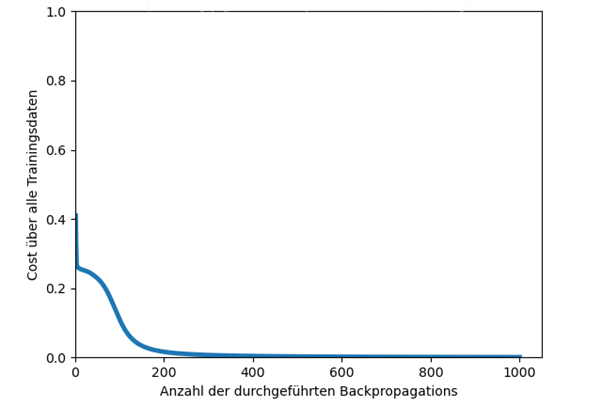
\includegraphics{pictures/cost_plot_teilbarkeit.png}
	\begingroup
	\captionof{figure}{Plot der Cost-Entwicklung für die Trainingsdaten (neuer Wert nach jedem Durchlauf der Backpropagation)}
	\endgroup


	\subsection{Die Musik}
	
	Zuerst haben wir nach einem einfachen Lied gesucht, das eine klare Struktur hat und nicht oder kaum von dieser abweicht. Dabei sind wir auf das Präludium Nr. 1 aus dem Wohltemperierten Klavier von Johannes Sebastian Bach gestoßen.
	
	\vspace{1.25ex}
	\begingroup
	\noindent 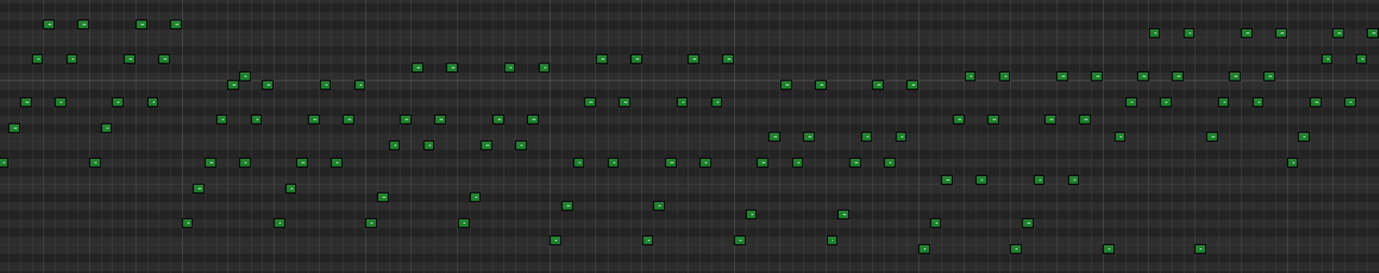
\includegraphics{"pictures/prel_1_org.png"}
	\captionof{figure}{Darstellung des Originalliedes} \label{fig:prel_1_org}
	\endgroup
	\vspace{1.25ex}
	
	Wie man in Abbildung \ref{fig:prel_1_org} sehen kann, werden in diesem Stück fast nur gebrochene Akkorde gespielt. Dabei bleibt das Muster, mit dem die Akkorde gebrochen werden, immer gleich. Außerdem wir jeder Akkord einmal wiederholt. Die KI muss also erkennen, wie das Muster funktioniert, mit dem die Akkorde gebrochen werden. Zusätzlich muss die KI erkennen, welche Akkorde und Akkordreihenfolgen (Kadenzen) verwendet werden.
	
	\vspace{1.25ex}
	\begingroup
	\noindent 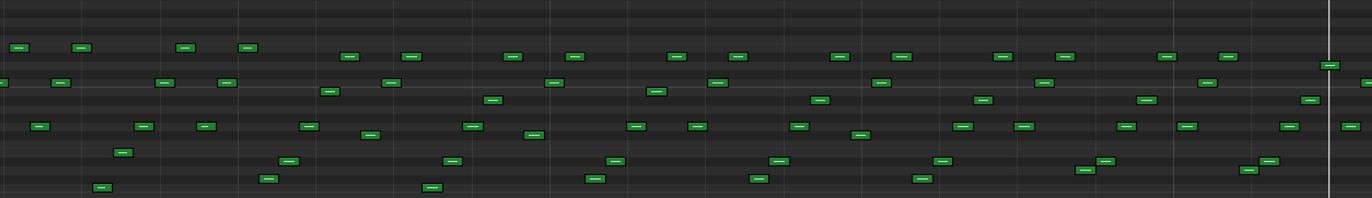
\includegraphics{"pictures/prel_1_ki.png"}
	\captionof{figure}{Darstellung des von der KI generierten Originalliedes} \label{fig:prel_1_ki}
	\endgroup
	\vspace{1.25ex}
	
	Man kann in Abbildung \ref{fig:prel_1_ki} erkennen, dass die KI das Muster gefunden hat, jedoch nur das grundlegende, wodurch das Ergebnis sehr repetitiv ist. Außerdem war sie nicht in der Lage, die Akkorde und Kadenzen des Stückes genau zu erkennen. Die Fehler sind zwar sehr klein, meist nur ein oder zwei Halbtöne daneben, führen aber dazu, dass das Lied für das menschliche Gehör dissonant klingt.
	
\section{Diskussion} \label{Diskussion}
	
	Nach einiger Überlegung haben wir mehrere Möglichkeiten gefunden, unser neuronales Netzwerk zu verbessern. Eine Möglichkeit wäre es, unseren Computer einfach länger rechnen zu lassen, vielleicht auch mehrere Computer zu benutzen oder ein schnelleres Programm zu programmieren, zum Beispiel, indem unklare Definitionen und unnötige Variablen vermieden werden. Außerdem ist es möglich, noch mehr Trainingsdaten zu generieren oder die vorhandenen Trainingsdaten effizienter zu gestalten, zum Beispiel durch das Berechnen der Anzahl an Noten (Inputs), die zur eindeutigen Vorhersage notwendig sind (\enquote{Musikalisches Gedächtnis}).
	
	Wir arbeiten im Moment auch an Unsupervised Learning. Unsupervised Learning ist besonders, da man damit eine Künstliche Intelligenz trainieren kann, ohne Label oder die richtigen Outputs zu den Input vorgeben zu müssen. Da er leicht mit der von uns bereits programmierten Struktur und Technik umsetzbar sein sollte, ist uns vor allem die Vorgehensweise mit einem Autoencoder ins Auge gefallen. Dieser funktioniert, indem ein Neuronales Netzwerk $x$ viele Noten als Inputs bekommt, im Hidden Layer aber weniger Neuronen hat. Als Output soll das Netzwerk dann versuchen, etwas möglichst ähnliches zum Input auszugeben. Da das Neuronale Netzwerk aufgrund der beschränkten Anzahl an Neuronen im Hidden Layer jedoch nicht einfach bei jedem Lied eins zu eins die Noten übertragen kann, muss es sogenannte Features, vergleichbar mit Mustern, in den gegebenen Trainingsdaten, in unserem Fall Liedern, finden, und diese über den Hidden Layer weiterleiten. Dieses Vorgehen ist ähnlich zu dem des menschlichen Gehirns, das sich zum Beispiel beim ersten Ansehen eines Schachbretts merkt, dass es ein $8\times8$ Feld mit immer abwechselnd schwarz und weißen Feldern ist, und nicht jeden einzelnen \enquote{Pixel}, also Lichtpunkt. In unserem Fall gäbe es voraussichtlich Features, die zum Beispiel das Tempo, die Dichte an Noten, die Art der Tonleiter, u.\,Ä bestimmen, jedoch meist nicht intuitiv verständlich sind, da sie von der KI selbst bestimmt werden. Wenn man nun damit ein Lied generieren möchte, kann man alle Layers vor diesem Hidden Layer weglassen und diesen zum Input Layer machen. So kann man nach Belieben die Werte der Features verändern und bekommt immer andere, (wahrscheinlich) komplett originale Lieder. [\hyperref[src:5]{5}]
	
	Eine andere Lösung könnte auch eine andere Art von neuronalem Netzwerk sein -- denn wir haben uns auf Deep Learning konzentriert, doch es gibt sehr viele andere Varianten. Außerdem gibt es die Möglichkeiten, mehr oder weniger Biases pro Layer zu benutzen, $\epsilon$ dynamisch anpassen zu lassen, und sogar die Struktur des Netzwerkes automatisch optimieren zu lassen. Man könnte auch unsupervised Learning probieren. Auch könnte es möglich sein, die Backpropagation so zu optimieren, dass sie z.B. vorausdenkt und so flache Plateaus verhindert werden. Der Zeitrahmen hat leider nicht gereicht, diese Dinge weiter zu recherchieren, jedoch wäre es eine Option für die Zukunft.
	
	Wir hatten auch eine Idee, wie man auf unserem Projekt aufbauen könnte: Man könnte versuchen, Google Deep Dream nachzuprogrammieren, aber nicht auf Bilder, sondern auf Lieder anzuwenden. Aber wie funktioniert Deep Dream überhaupt?
	
	\vspace{1.25ex}
	\begingroup
	\noindent 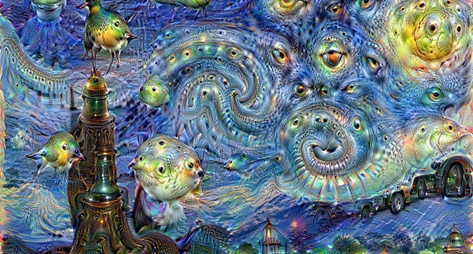
\includegraphics[width=\linewidth]{pictures/deep_dream.png}
	\captionof{figure}{Ein Beispiel für ein Deep Dream Bild ${}^{\hyperref[src:deep_dream]{[7]}}$}
	\label{fig:deep_dream}
	\endgroup
	\vspace{1.25ex}
	
	Zuerst programmiert man ein neuronales Netzwerk, das bestimmte Bilder klassifizieren kann (in Abbildung \ref{fig:deep_dream} wahrscheinlich Vögel). Um Vögel zu erkennen, muss das neuronale Netzwerk bestimmte Muster erkennen, die in Bildern von Vögeln vorkommen. Danach gibt man dem neuronalen Netzwerk ein neues Bild als Input. Nun guckt man für alle Neuronen eines bestimmten Layers, ob sie eine hohe Aktivierung haben. Wenn die Aktivierung einen bestimmten Schwellenwert überschreitet, bedeutet das, dass das neuronale Netzwerk ein Muster erkennt, welches in Bildern von Vögeln gefunden werden kann. Anschließend kann man mit Hilfe der Backpropagation ausrechnen, wie man das Bild (den Input) verändern kann, damit die Aktivierung, die den Schwellenwert überschritten hat, noch größer wird. Somit wird das Bild \enquote{vogeliger}. Auf Lieder angewandt könnte man so zum Beispiel klassische Lieder \enquote{jazziger} machen.

\newpage
\section{Quellen}

\subsection{Bücher}
\begin{itemize}
	\item [1] \label{src:1} Andreas Zell:\\[0.25ex]
	Simulation Neuronaler Netze, Addison Wesley (Deutschland) GmbH, 1994\\
	letzter Zugriff: 02.01.2021
\end{itemize}

\subsection{Internetquellen}
\begin{itemize}
	\item [2] \label{src:2} Grant Sanderson:\\[0.25ex]
	Neural Networks-Series\\
	(\href{https://www.youtube.com/playlist?list=PLZHQObOWTQDNU6R1\_67000Dx\_ZCJB-3pi}{https://www.youtube.com/playlist?list=PLZHQObOWTQDNU6R1\_67000Dx\_ZCJB-3pi})\\
	letzter Zugriff: 03.01.2021
	\item [3] \label{src:3} Brotcrunsher:\\[0.25ex]
	Neuronale Netze -- Backpropagation\\
	(\href{https://www.youtube.com/watch?v=YIqYBxpv53A}{https://www.youtube.com/watch?v=YIqYBxpv53A},\\
	\href{https://www.youtube.com/watch?v=EAtQCut6Qno}{https://www.youtube.com/watch?v=EAtQCut6Qno})\\
	letzter Zugriff: 31.12.2020
	\item [4] \label{src:4} Fabian Beck \& Günter Daniel Rey:\\[0.25ex]
	Neuronale Netze: Eine Einführung -- Backpropagation -- Probleme\\
	(\href{http://www.neuronalesnetz.de/backpropagation5.html}{http://www.neuronalesnetz.de/backpropagation5.html})\\
	Letzter Zugriff: 04.01.2021\\[0.25ex]
	Neuronale Netze: Eine Einführung -- Backpropagation -- Lösungen\\
	(\href{http://www.neuronalesnetz.de/backpropagation6.html}{http://www.neuronalesnetz.de/backpropagation6.html})\\
	Letzter Zugriff: 04.01.2021
	\item [5] \label{src:5} CodeParade:\\[0.25ex]
	Computer Generates Human Faces\\
	\href{https://www.youtube.com/watch?v=4VAkrUNLKSo}{https://www.youtube.com/watch?v=4VAkrUNLKSo}\\
	Letzter Zugriff: 27.02.2021\\[0.25ex]
	Generating Songs With Neural Networks (Neural Composer)\\
	\href{https://www.youtube.com/watch?v=UWxfnNXlVy8}{https://www.youtube.com/watch?v=UWxfnNXlVy8}\\
	Letzter Zugriff: 27.02.2021
\end{itemize}

\subsection{Julia-Packages}
\begin{itemize}
	\item \label{src:midi}George Datseris und Joel Hobson:\\[0.25ex]
	MIDI, seit Aug 23, 2015\\
	(\href{https://github.com/JuliaMusic/MIDI.jl}{https://github.com/JuliaMusic/MIDI.jl})
	\item \label{src:pyplot} Steven G. Johnson\\[0.25ex]
	PyPlot, seit Nov 18, 2012\\
	(\href{https://github.com/JuliaPy/PyPlot.jl}{https://github.com/JuliaPy/PyPlot.jl}) 
	\item \label{src:jld} Simon Kornblith und Tim Holy:\\[0.25ex]
	JLD, seit Aug 23, 2015\\
	(\href{https://github.com/JuliaIO/JLD.jl}{https://github.com/JuliaIO/JLD.jl}) 
\end{itemize}
	
\subsection{Midi-Dateien für Trainings-/Testdaten}
	\begin{itemize}
		\item \href{https://bitmidi.com/}{https://bitmidi.com/}
		\item \href{https://www.midiworld.com/files/}{https://www.midiworld.com/files/}
	\end{itemize}

\subsection{Abbildungen}
\begin{itemize}
	\item[6] \label{src:num_4} \href{https://www.heise.de/select/ix/2017/9/1504455013673842/contentimages/avr.tut.ml-python-2.B1.jpg}{https://www.heise.de/select/ix/2017/9/1504455013673842/contentimages/avr.tut.ml-python-2.B1.jpg}
	\item[7] \label{src:deep_dream} \href{https://deepdreamgenerator.com/\#gallery}{https://deepdreamgenerator.com/\#gallery} \textrightarrow Unterkategorie \enquote{DEEP DREAM}
\end{itemize}
Wenn nicht anders angegeben, sind Abbildungen selbst erstellt.

\section{Unterstützungsleistungen}

\textbf{Prof. Dr. Bernd Blasius}\\
Hilfe beim / Ideen für das/die:
\begin{itemize}
	\item Bugfixing (Beseitigung von Softwarefehlern)
	\item Speichern von Weights in multidimensionalen Arrays statt Dictionaries\\
	\textrightarrow Performance Verbesserung\\
	\textrightarrow Verkürzung des Programms
	\item Genauere Definition von Arrays, um den Datentyp Any zu vermeiden
	\textrightarrow Performance Verbesserung
\end{itemize}

\end{document}